\documentclass[12pt, a4paper]{article}

\usepackage[utf8]{inputenc}
\usepackage[ngerman]{babel}
\usepackage[T1]{fontenc}
\usepackage{float}
\usepackage{graphicx}
\graphicspath{ {./GUI imgs/} }
\usepackage{pifont}% http://ctan.org/pkg/pifont
\title{Pflichtenheft}

\begin{document}

\maketitle
\pagebreak
\tableofcontents
\pagebreak

\section{Zielbestimmung}
\subsection{Musskriterien}
\paragraph{Allgemein}
\begin{itemize}
	\item /M01/ Akteure: Gast, Nutzer, wobei Gast \textless  Nutzer (a \textless b bedeutet b erbt von a).
	\item /M02/ Die Bibliothek soll von Nutzern, also von Lehrstuhlmitarbeitern und Studenten benutzt werden.
	\item /M03/ Es gibt drei Gruppen von Nutzern mit verschiedenen Rechten: Lehrstuhlmitarbeiter, Studenten und Administratoren, wobei Studenten \textless Lehrstuhlmitarbeiter \textless Administratoren
	\item /M04/ Jeder Nutzer soll zu genau einer Gruppe gehören.
	\item /M05/ Studenten sollen nur zur Gruppe Studenten gehören.
	\item /M06/ Lehrstuhlmitarbeiter sollen entweder zur Gruppe Lehrstuhlmitarbeiter oder Administratoren gehören.
	\item /M07/ Es muss immer mindestens ein Nutzer innerhalb der Gruppe Administratoren existieren
	\item /M08/ Eine intuitive, rechnergestützte GUI soll umgesetzt werden
	\item /M09/ Die Produktleistungswerte (siehe 6 Produktleistungen) sollen eingehalten werden.
	\item /M10/ Alle Produktdateneinträge sollen persistent gespeichert werden.
	\item /M11/ Das System soll von jedem Rechnersystem des Lehrstuhls erreichbar sein.
	\item /M12/ Mehrere Nutzer können gleichzeitig auf die Software zugreifen.
	\item /M13/ Das System soll Bücher, Zeitschriften und Datenträger aller Art sowie elektronische Medien verwalten können.
	\item /M14/ Automatisches Versenden von Mahnungen und Verwarnungen ist möglich.
	\item /M15/ Automatisches Versenden von Rückgabeerinnerungen ist möglich.
\end{itemize}
\paragraph{jeder Gast kann ...}
\begin{itemize}
	\item /M16/ eine Suche nach einem Medium über Metadaten ausführen.
	\item /M17/ eine Suche nach einem Medium über den Inhalt ausführen, falls  dieser im System elektronisch vorhanden ist.
\end{itemize}
\paragraph{jeder Nutzer kann ...}
\begin{itemize}
	\item /M18/ sich einloggen.
	\item /M19/ sich ausloggen.
	\item /M20/ physische Medien ausleihen.
	\item /M21/ physische Medien vormerken.
	\item /M22/ physische Medien verlängern.
	\item /M23/ physische Medien zurückgeben.
	\item /M24/ digitale Medien ansehen.
	\item /M25/ digitale Medien herunterladen.
\end{itemize}
\paragraph{jeder Nutzer aus der Gruppe Lehrstuhlmitarbeiter kann ...}
\begin{itemize}
	\item /M26/ eine Übersicht über die aktuell ausgeliehenen Medien erhalten.
	\item /M27/ ein neues Medium hinzufügen.
	\item /M28/ Daten von Medien ändern.
	\item /M29/ einen neuen Nutzer zur Gruppe Studenten hinzufügen.
	\item /M30/ Daten von Nutzern aus der Gruppe Studenten ändern.
\end{itemize}
\paragraph{jeder Nutzer aus der Gruppe Administratoren kann ...}
\begin{itemize}
	\item /M31/ einen neuen Nutzer zur Gruppe Studenten, Lehrstuhlmitarbeiter oder Administratoren hinzufügen.
	\item /M32/ Daten von allen Nutzern ändern.
	\item /M33/ Rechte von Gruppen ändern.
\end{itemize}
\subsection{Wunschkriterien}
\begin{itemize}
	\item /W01/ Einführung von neuen Medien-Kategorien durch Lehrstuhlmitarbeiter.
	\item /W02/ Explizite Änderung der Ausleihdauer für jede einzelne Ausleihe.
	\item /W03/ System für das Zurücksetzen von Passwörtern.
	\item /W04/ Skalierbarkeit vom System, um es leicht um weitere Lehrstühle erweitern zu können.
	\item /W05/ Möglichkeit des Hinzufügens neuer Gruppen durch Administratoren
\end{itemize}
\subsection{Abgrenzungskriterien}
\begin{itemize}
	\item /A01/ keine Unterstützung für Touchscreens.
	\item /A02/ kein Fokus auf das Sicherheitssystem des Systems,  Immunität des Systems gegen Hacker-Angriffe ist also unter Umständen nicht gewährleistet.
\end{itemize}
\pagebreak

\section{Produkteinsatz}
\subsection{Anwendungsbereiche}
Der Dienst wird für die Benutzung der Lehrstuhlbibliothek für die Softwaretechnologie verwendet.  Das System soll mehrere Optionen anbieten, wie z.B Suche nach den Medien, Ausleihe, Verlängern und Monitoring. Das System verwaltet sowohl physische als auch digitale Medien.
\subsection{Zielgruppen}
Personengruppen, die entweder Lehrstuhlmitarbeiter oder Studenten sind, können die Bibliothek benutzen. Gäste können nur nach den Medien suchen.
\subsection{Betriebsbedingungen}
Dieses System soll folgende Bedingungen erfüllen:
\begin{itemize}
\item Betriebsdauer: 24 Stunden täglich
\item Wartungsfrei
\item Die Sicherung der Datenbank muss manuell vom Administrator durchgefuhrt werden
\item Das System soll von jedem Rechnersystem des Lehrstuhls erreichbar sein
\end{itemize}
\pagebreak

\section{Technische Produktumgebung}
Das Produkt besteht aus Client und Server.
\subsection{Software}
\textit{Server}: Ubuntu Server 18.04 LTS, MariaDB 10.4 \\
\textit{Client}: Browser
\subsection{Hardware}
\textit{Server}: PC \\
\textit{Client}: Browser-fähiges Gerät mit Grafikbildschirm
\subsection{Orgware}
Einbindung des Servers in das Lehrstuhlnetzwerk
\subsection{Produktschnittstellen}
Keine

\pagebreak

\section{Produktfunktionen}

Die Software soll in der Lage sein, die Verwaltung einer Bibliothek durchzuführen. Hier werden die Punkte aus dem Lastenheft erneut aufgeführt und sofern weiter möglich näher erklärt.
\begin{itemize}
	\item /LF10/ das Ausleihen und Zurückgeben von physischen Medien unterschiedlicher Arten ist möglich

		Das Ausleihen und Zurückgeben erfolgt über die Eingabe der Medien-ID oder das Auswählen des Mediums in der Suche, bzw. bei der Rückgabe durch Auswahl im Account.
		Bei digitalen Medien ist keine Zurückgabe notwendig, hier wird nur der Zugriff in der Ausleihhistorie vermerkt.
	\item /LF20/ digitale Medien sind zum Download/zur Einsicht verfügbar

	Digitale Medien sind über die Suche aufrufbar, dem Nutzer soll dann die Wahl bleiben, ob er das Medium vollständig herunterladen oder sich nur kurzfristig anzeigen lassen möchte
	\item /LF30/ Mahnungen und Rückgabeerinnerungen werden automatisch versendet

	Die Bestätigung des Versands dieser Erinnerungen soll in der Monitoringübersicht einsehbar sein.

	\item /LF40/ Lehrstuhlmitarbeiter können eine Übersicht über die aktuell ausgeliehenen Medien erhalten

	\item /LF50/ das Ausleihen ist nur Studenten und Mitarbeitern möglich

	Dies wird über die Gruppenrechte kontrolliert, Gastnutzer erhalten die notwendigen Rechte nicht.
	\item /LF60/ Ausleihen können verlängert werden, wenn das Medium nicht vorbestellt ist
	\item /LF70/ eine Mediensuche ist über sämtliche Metadaten und den Inhalt möglich

	Die Metadaten sind unter \textit{5 Produktdaten /PD11/} aufgeführt
\end{itemize}
\pagebreak

\section{Produktdaten}
\begin{itemize}
	\item /LD10/ die Bibliothek wird auf längere Sicht <50.000 Medien umfassen
	\item /PD11/ die Metadaten eine Mediums sind Name, Veröffentlichungsdatum, Autor, Kategorie/Genre und Verfügbarkeit sowie optional der Verlag
\end{itemize}

Die innerhalb eines Jahres voraussichtlich abzuspeichernden Daten sind:
\begin{itemize}
	\item /LD20/ Nutzer- und Gruppeninformationen mit <1.000 Einträgen
	\item /PD21/ Nutzerinformationen umfassen Namen, Logininformationen, Mitarbeiter-/Matrikelnummer, Gruppenzugehörigkeit und aktuelle Ausleihen
	\item /PD22/ Gruppendaten umfassen den Namen, Rechte zur Ausleihe und Verwaltung und die mögliche Ausleihdauer
	\item /LD30/ Ausleihe- und Monitoringdaten mit <50.000 Einträgen
	\item /PD31/ die Ausleihdaten beinhalten die Ausleihhistorie aller Medien und der zugehörigen Nutzer, sowie alle aktuellen Ausleihen
	\item /PD32/ die Monitoringdaten beinhalten die Informationen zu gezahlten und ausstehenden Mahngebühren
\end{itemize}
\pagebreak

\section{Produktleistungen}
Solange die unter "5 Produktdaten" genannten Datenmengen nicht überschritten werden, gelten die Leistungsansprüche aus dem Lastenheft. Ansonsten steigen die zu akzeptierenden Leistungseinbußen proportional zu der zusätzlichen Datenmenge.
\begin{itemize}
	\item /LL10/ Anfragezeiten von <2sec für Mediensuchen
	\item /LL20/ Anfragezeiten von <1sec für Nutzer- und Gruppensuchen
	\item /LL30/ Anfragezeiten von <2sec für Ausleihe- und Monitoringdaten
	\item /LL40/ Zeitliche Fristen sind auf 24-Stunden-Basis beschränkt, also reicht eine zeitliche Genauigkeit von 1 min
	\item /LL50/ Abmahngebühren müssen in korrekten Euro-Werten angegeben werden
\end{itemize}
\pagebreak

\section{Benutzeroberfläche}
\begin{itemize}
	\item Startseite
\end{itemize}
\begin{figure}[h]
	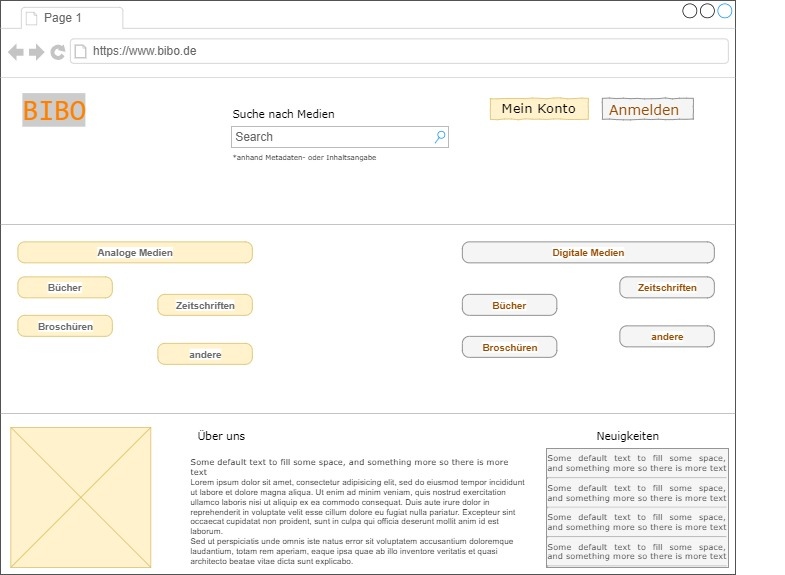
\includegraphics[width=\textwidth]{GUIs/startseite.jpg}
	\caption{Startseite}
	\label{fig:startseite}
\end{figure}
\pagebreak
\begin{itemize}
	\item Benutzer meldet sich an
\end{itemize}
\begin{figure}[h]
	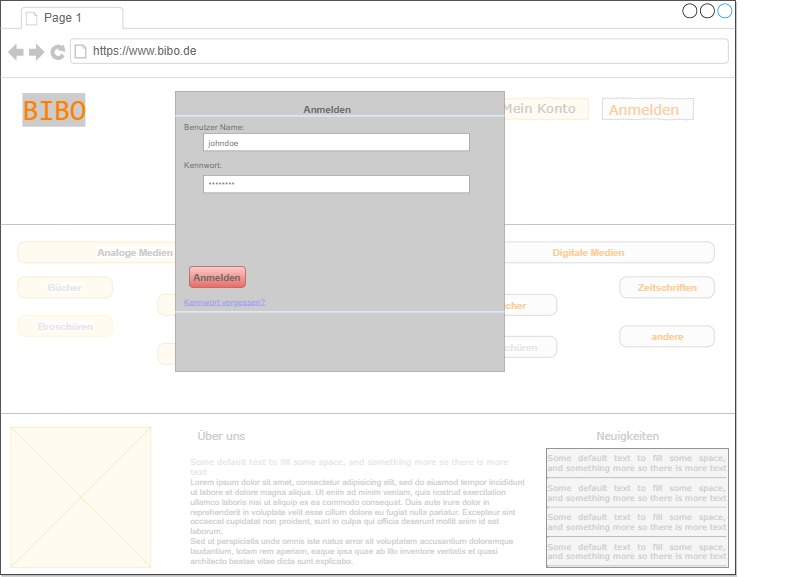
\includegraphics[width=\textwidth]{GUIs/anmelden.jpg}
	\caption{Benutzer meldet sich an}
	\label{fig:anmeldung}
\end{figure}
\pagebreak
\begin{itemize}
	\item Gast stellt Suchtanfragen
\end{itemize}
\begin{figure}[h]
	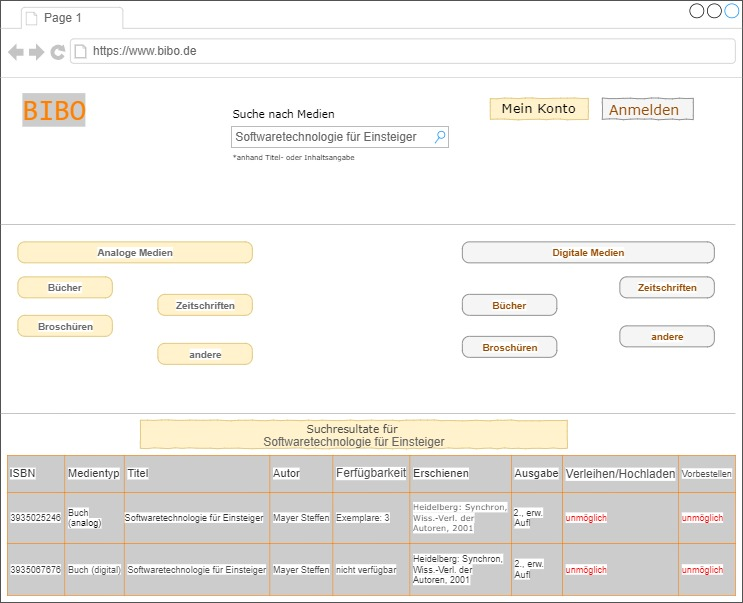
\includegraphics[width=\textwidth]{GUIs/such_Gast.jpg}
	\caption{Gast stellt Suchtanfragen}
	\label{fig:suchtanfragen_gast}
\end{figure}
\pagebreak
\begin{itemize}
	\item Angemeldeter Nutzer stellt Suchtanfragen
\end{itemize}
\begin{figure}[h]
	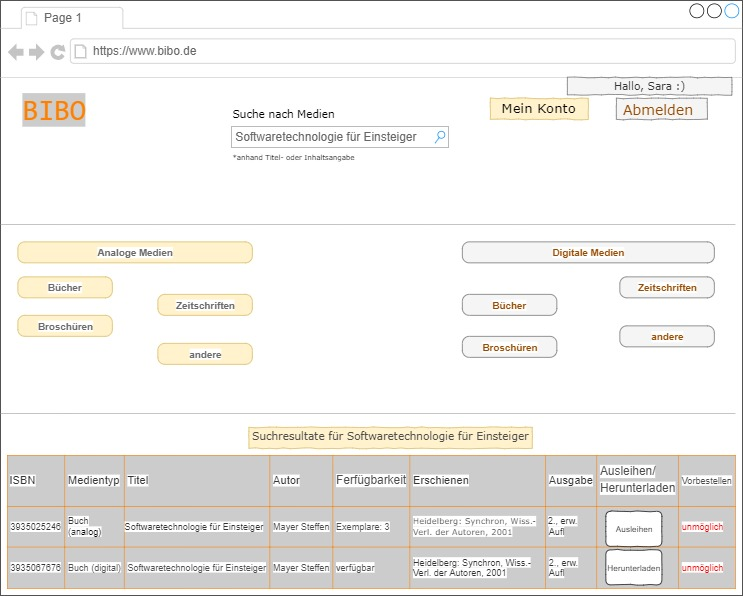
\includegraphics[width=\textwidth]{GUIs/such_angemNutzer.jpg}
	\caption{Angemeldeter Nutzer stellt Suchanfragen}
	\label{fig:suchtanfragen_angem_nutzer}
\end{figure}
\pagebreak
\begin{itemize}
	\item Mein Konto
\end{itemize}
\begin{figure}[h]
	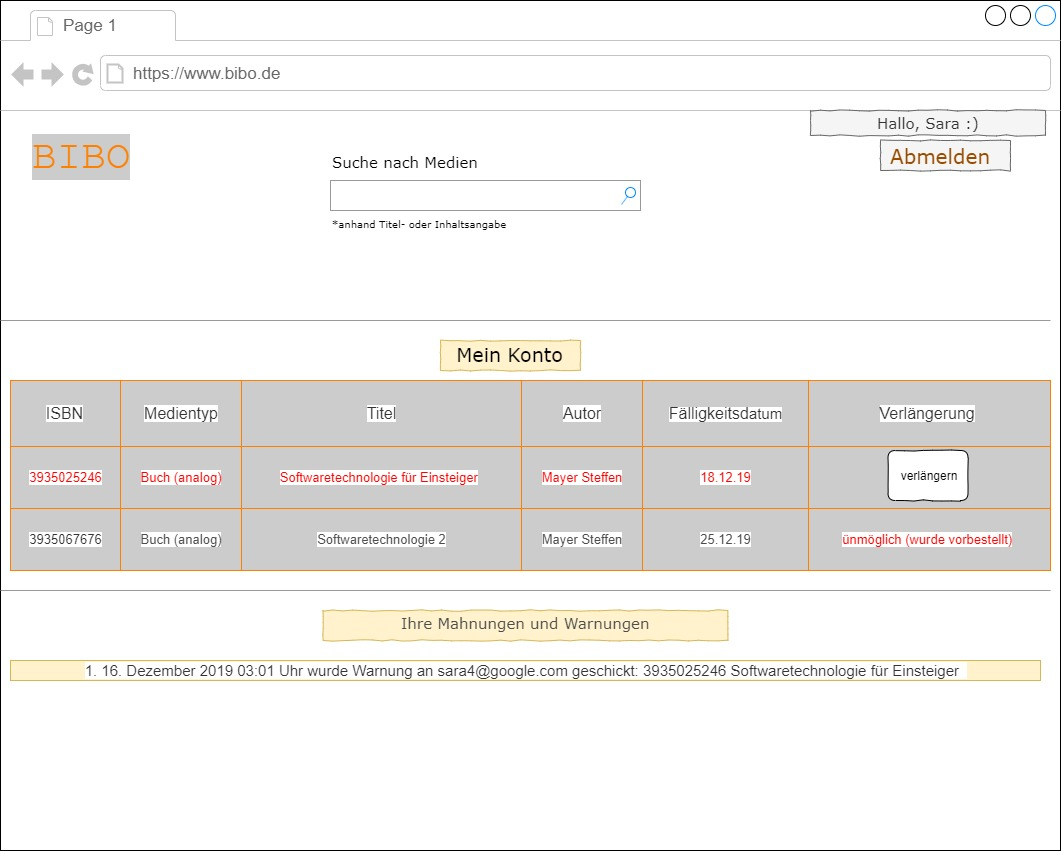
\includegraphics[width=\textwidth]{GUIs/mein_Konto.jpg}
	\caption{Mein Konto}
	\label{fig:mein_konto}
\end{figure}
\pagebreak
\begin{itemize}
	\item Lehrstuhlmitarbeiter im System
\end{itemize}
\begin{figure}[h]
	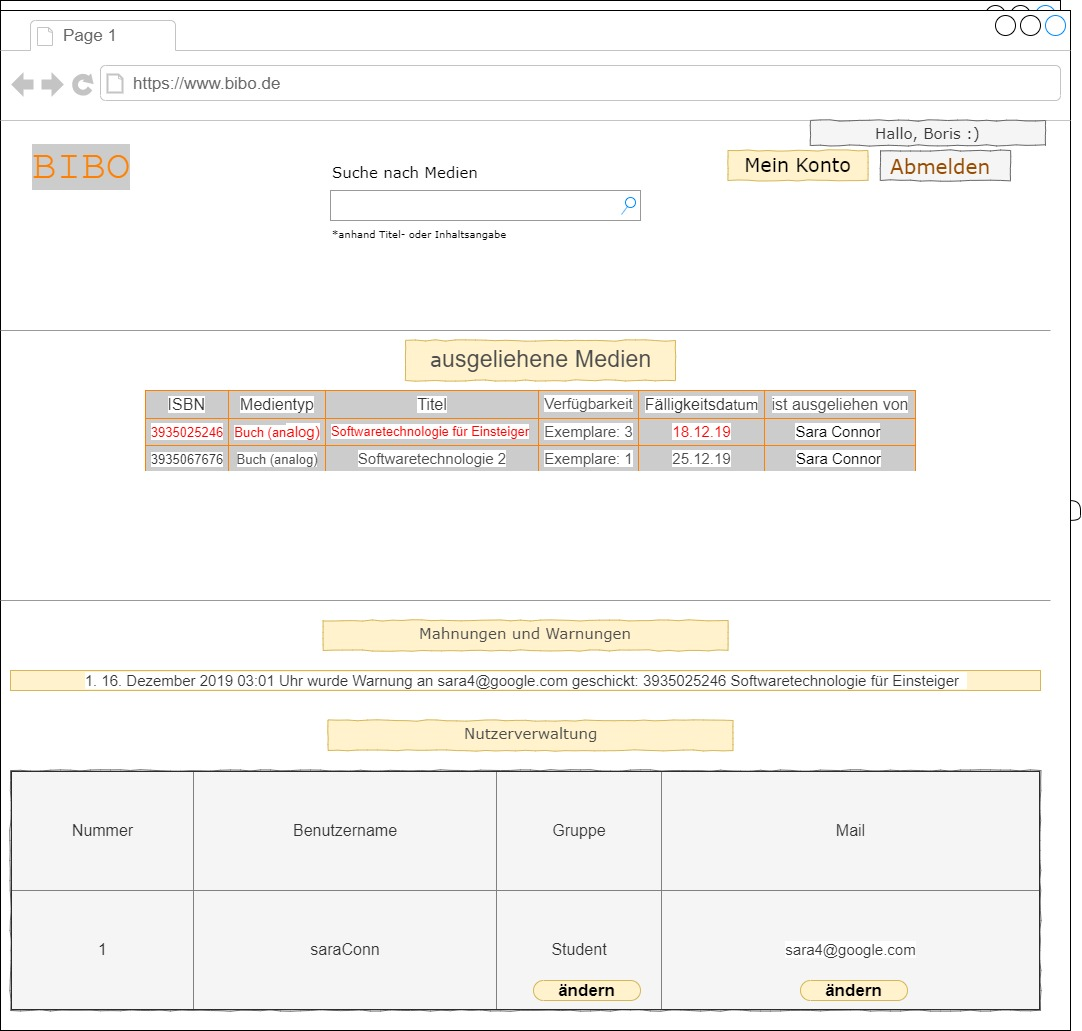
\includegraphics[width=\textwidth]{GUIs/ang_ansicht.jpg}
	\caption{Lehrstuhlmitarbeiter im System}
	\label{fig:ang_ansicht}
\end{figure}
\pagebreak


\section{Qualitätsanforderungen}
\newcommand{\xmark}{\ding{55}}%
\begin{table}[h]
	\centering
\begin{tabular}{ || c | c | c | c | c || }
	\hline
	Produktqualität & sehr gut & gut & normal & nicht relevant  \\ \hline
	\textbf{Funktionalität} \\  \hline
	Angemessenheit & & \xmark &  &  \\ \hline
	Richtigkeit &  & \xmark &  &  \\ \hline
	Interoperabeltät &  & \xmark &  &  \\ \hline
	Ordnungsgemäßigkeit &  & \xmark &  &  \\ \hline
	Sicherheit &  & \xmark &  &  \\ \hline
	\textbf{Zuverlässigkeit} \\ \hline
	Reife & & & \xmark  &  \\ \hline
	Fehlertoleranz & & & \xmark  &  \\ \hline
	Wiederherstellbarkeit & & & \xmark  &  \\ \hline
	\textbf{Benutzbarkeit} \\ \hline
	Verständlichkeit &  \xmark & &  &  \\ \hline
	Erlernbarkeit &  &\xmark &  &  \\ \hline
	Bedienbarkeit &  \xmark & &  &  \\ \hline
	\textbf{Effizienz} \\ \hline
	Zeitverhalten &  &  & \xmark  &  \\ \hline
	Verbrauchsverhalten &  &  & \xmark  &  \\ \hline
	\textbf{Änderbarkeit} \\ \hline
	Analysierbarkeit &  &  & \xmark  &  \\ \hline
	Modifizierbarkeit &  &  & \xmark  &  \\ \hline
	Stabilität &  \xmark & & &  \\ \hline
	Prüfbarkeit &  &  & \xmark  &  \\ \hline
	\textbf{Übertragbarkeit} \\ \hline
	Anpassbarkeit &   & \xmark & &  \\ \hline
	Installierbarkeit &  &  \xmark & & \\ \hline
	Konformität &  &   \xmark & & \\ \hline
	Austauschbarkeit &  &  \xmark & & \\ \hline
\end{tabular}
\caption{Qualitätszielbestimmung}
\label{table:qualitätsanforderungen}
\end{table}

\pagebreak

\section{Globale Testszenarien/Akzeptanztestfälle}
\begin{table}[H]
	\begin{tabular}{p{1.2cm}|p{6.5cm}|p{5.5cm}}
		\textbf{Id} & \textbf{Beschreibung} & \textbf{Erwartetes Ergebnis}\\
		\hline
		/T01/ & Zugang auf die Webseite von außerhalb des Lehrstuhls & Seite nicht verfügbar\\
		\hline
		/T02/ & Einloggen mit inkorrekten Daten & Einloggen fehlgeschlagen\\
		\hline
		/T03/ & Einloggen mit korrekten Daten & Einloggen erfolgreich\\
		\hline
		/T04/ & Ausloggen & Ausloggen erfolgreich\\
		\hline
		/T05/ & mehrere Nutzer greifen gleichzeitig auf die Seite zu & Kein Absturz\\
		\hline
		/T06/ & Hinzufügen eines Studenten zur Gruppe Studenten durch Lehrstuhlmitarbeiter & Der Student gehört zur Gruppe Studenten\\
		\hline
		/T07/ & Löschen des letzten Administrators durch diesen Administrator & Fehler; Löschen darf nicht möglich sein\\
		\hline
		/T08/ & Hinzufügen eines Lehrstuhlmitarbeiters zur Gruppe Administratoren durch Administrator & Der Lehrstuhlmitarbeiter wird Administrator\\
		\hline
		/T09/ & Löschen eines Administrators durch Administrator & der Nutzer wird zur Gruppe Lehrstuhlmitarbeiter gehören\\
		\hline
		/T10/ & Hinzufügen eines Studenten zur Gruppe Administratoren & Fehlermeldung\\
		/T11/ & Hinzufügen eines Lehrstuhlmitarbeiters durch Administrator zur Gruppe Studenten & Fehlermeldung\\
		\hline
		/T12/ & Hinzufügen eines Buches mit Titel  'Buch1'  (ohne andere Metadaten) zum System & Fehlermeldung bei der Validierung\\
		\hline
		/T13/ & Hinzufügen eines Buches mit Titel  'Buch1'  (mit anderen Metadaten) zum System & Ein Buch vom Titel  'Buch1'  wurde zum Katalog hinzugefügt\\
		\hline
		/T14/ & Hinzufügen eines E-Books mit Titel  'Buch2'  und Inhalt  '...lorem ipsum'  (mit anderen Metadaten) zum System & Ein E-Book wurde zum Katalog hinzugefügt\\
    \end{tabular}
\end{table}

\begin{table}
	\begin{tabular}{p{1.2cm}|p{6.5cm}|p{5.5cm}}

		\hline
		/T15/ & Suchen über das Wort  'Buch'  & Zwei Einträge gefunden\\
		/T16/ & Suchen über das Wort  'Buch1'  & Ein Eintrag gefunden\\
		\hline
		/T17/ & Suchen über das Wort  'lorem'  & Ein Eintrag gefunden\\
		\hline
		/T18/ & Anschauen von E-Book  'Buch2'  & Anschauen war möglich\\
		\hline
		/T19/ & Herunterladen von E-Book  'Buch2'  & Herunterladen wurde erfolgreich abgeschlossen\\
		\hline
		/T20/ & Ausleihen von Buch  'Buch1'  & Ausleihe erfolgreich abgeschlossen\\
		\hline
		/T21/ & Änderung der Ausleihedauer für die Gruppe Studenten auf 3 Tage durch Administrator & Änderung erfolgreich\\
		\hline
		/T22/ & Es ist drei Tage vor der erwarteten Abgabe für  'Buch1' & Versand einer Rückgabeerinnerung zum Studenten über 'Buch1' \\
		\hline
		/T23/ & Änderung des Titels von  'Buch1'  zu  'Buch3' durch einen Lehrstuhlmitarbeiter & Änderung erfolgreich\\
		\hline
		/T24/ & Abrufen einer Übersicht über die aktuell ausgeliehenen Medien & korrekte Daten werden angezeigt ( 'Buch 3'  ist ausgeliehen)\\
		\hline
		/T25/ & Vormerken des Buches 'Buch3' durch anderen Nutzer & Das Buch wurde vorgemerkt\\
		\hline
		/T26/ & Verlängern des Buches 'Buch3' & Verlängerung nicht möglich, weil es schon vorgemerkt wurde\\
		\hline
		/T27/ & das Ausleihdatum von  'Buch1'  ist vorbei & Versand einer Mahnung zum Student über  'Buch1'  mit der Strafangaben in Euros \\
		\hline
		/T28/ & Rückgabe von Buch  'Buch1'  & Rückgabe erfolgreich abgeschlossen\\
		\hline
		/T29/ & Abrufen einer Übersicht über die aktuell ausgeliehenen Medien & korrekte Daten angezeigt (leer)\\
		\hline
		/T30/ & [mehrere Medien hinzugefügt] Schicken einer Anfrage für ein Medium & Anfragezeit von \textless 2sec\\
		\hline
		/T31/ & [mehrere Nutzer hinzugefügt] Schicken einer Anfrage zu einem Nutzer & Anfragezeit von \textless 1sec\\
		\hline
		/T32/ & Schicken einer Anfrage für eine Gruppe & Anfragezeit von \textless 1sec\\
		\hline
		/T33/ & [mehrere Ausleihen durchgeführt] Schicken einer Anfrage für eine Ausleihe & Anfragezeit von \textless 2sec\\
    \end{tabular}
\end{table}
\pagebreak

\section{Glossar}
\textbf{Gast}
\\*
Eine Person, die keiner Nutzergruppe zugeordnet ist, oder keinen Bibiotheksaccount besitzt.
\\*
\textbf{Nutzer}
\\*
Ein angemeldeter Nutzer der Lehrstuhlbibliothek. Ist ein Überbegriff für $\rightarrow$ Studenten  und $\rightarrow$ Lehrstuhlmitarbeiter.
\\*
\textbf{Lehrstuhlmitarbeiter}
\\*
Ein Mitarbeiter des Lehrstuhls.
\\*
\textbf{Student}
\\*
Ein Student der Fakultät, der der Lehrstuhl angehört.
\\*
\textbf{Gruppe}
\\*
Eine abstrakte Entität, in der bestimmte $\rightarrow$Rechte zusammengefasst werden. Jeder $\rightarrow$Nutzer ist genau einer Gruppe zugeordnet.
\\*
\textbf{Rechte}
\\*
Befähigt einen Nutzer dazu, bestimmte Funktionen der Lehrstuhlbibliothek zu nutzen (zum Beispiel das →Ausleihen von →Medien).
\\*
\textbf{Administrator}
\\*
Ist ein $\rightarrow$Lehrstuhlmitarbeiter, der dazu berechtigt ist, die $\rightarrow$Lehrstuhlbibliothek zu administrieren.
\\*
\textbf{Mahnung}
\\*
Wird abgeschickt, wenn ein $\rightarrow$Nutzer der $\rightarrow$Lehrstuhlbibliothek ein $\rightarrow$Medium nicht zeitgerecht zurückgibt.
\\*
\textbf{Medium}
\\*
Ein Überbegriff für $\rightarrow$physische Medien und $\rightarrow$digitale Medien.
\\*
\textbf{physisches Medium}
\\*
Ist ein ausleihbares Medium. Beinhaltet Bücher, Zeitschriften, Datenträger und Broschhüren.
\\*
\textbf{digitales Medium}
\\*
Ist ein Sammelbegriff für alle Medien, die elektronisch in der Lehrstuhlbibliothek hinterlegt sind.
\\*
\textbf{Ausleihe}
\\*
Eine Tätigkeit, wobei unentgeldlich ein $\rightarrow$Medium von einem $\rightarrow$Nutzer für eine bestimmte Zeit benutzt werden kann. Nach Ablauf der Ausleihdauer muss das $\rightarrow$Medium zurückgegeben werden.
\\*
\textbf{Lehrstuhl}
\\*
Ist ein Teilgebiet der Universität.
\\*
\textbf{Lehrstuhlbibliothek}
\\*
Beschreibt die Gesamtheit der $\rightarrow$Medien des $\rightarrow$Lehrstuhles sowie das elektronische System zum Verwalten dieser Medien.
\\*
\textbf{Webseite/Seite}
\\*
Ist die Softwareoberfläche, mit der die $\rightarrow$ Lehrstuhlbibliothek von den $\rightarrow$ Nutzern benutzt werden kann.
\pagebreak

\end{document}
